% Word count: 852

\section{Technical Feasibility}
In order to asses the technical feasibility of this project three \textit{Proof of Concepts} (POCs) have been defined.

\begin{POC}
	\item \label{poc1} \textbf{Validation:} How will a restoration be validated? What criteria are needed for a backup to be deemed successful?
	\item \label{poc2} \textbf{User Rules:} How will a user use the system? Can the the implementation of a backup restoration be abstracted from the user by means of a user friendly frontend?
	\item \label{poc3} \textbf{Security:} How will the system deal with encrypted backups? Can the Jenkins server safely handle credentials and decrypt backups in order to perform the test restoration?
\end{POC}

	\subsection{\ref{poc1} Validation}
	\subsubsection{Work Carried Out}	
	In order to prove that validation of a backup can be achieved via Jenkins the following infrastructure was deployed:
	\begin{itemize}
		\item \textbf{Backup Server:} An EC2 instance on which a backup file was saved.
		\item \textbf{Restoration Server:} An EC2 instance with the MongoDB DBMS installed and running.
		\item \textbf{Jenkins Server.}
	\end{itemize}
	A Jenkins job was then configured to execute the following tasks:
	\begin{enumerate}
		\item Copy backup file from \textit{backup} server to \textit{restoration} server (sample MongoDB data used \citep{mongo});
		\item Import the backup file into MongoDB on \textit{restoration} server;
		\item Run a \textit{findAll} command on the MongoDB database to retrieve all entries;
		\item Print the entries to Jenkins console;
	\end{enumerate}
	A sample output of this job executing each of the steps above can be observed in \autoref{fig:poc1}.
	\begin{figure}[H]
		\caption{Backup Validation}
		\centering
		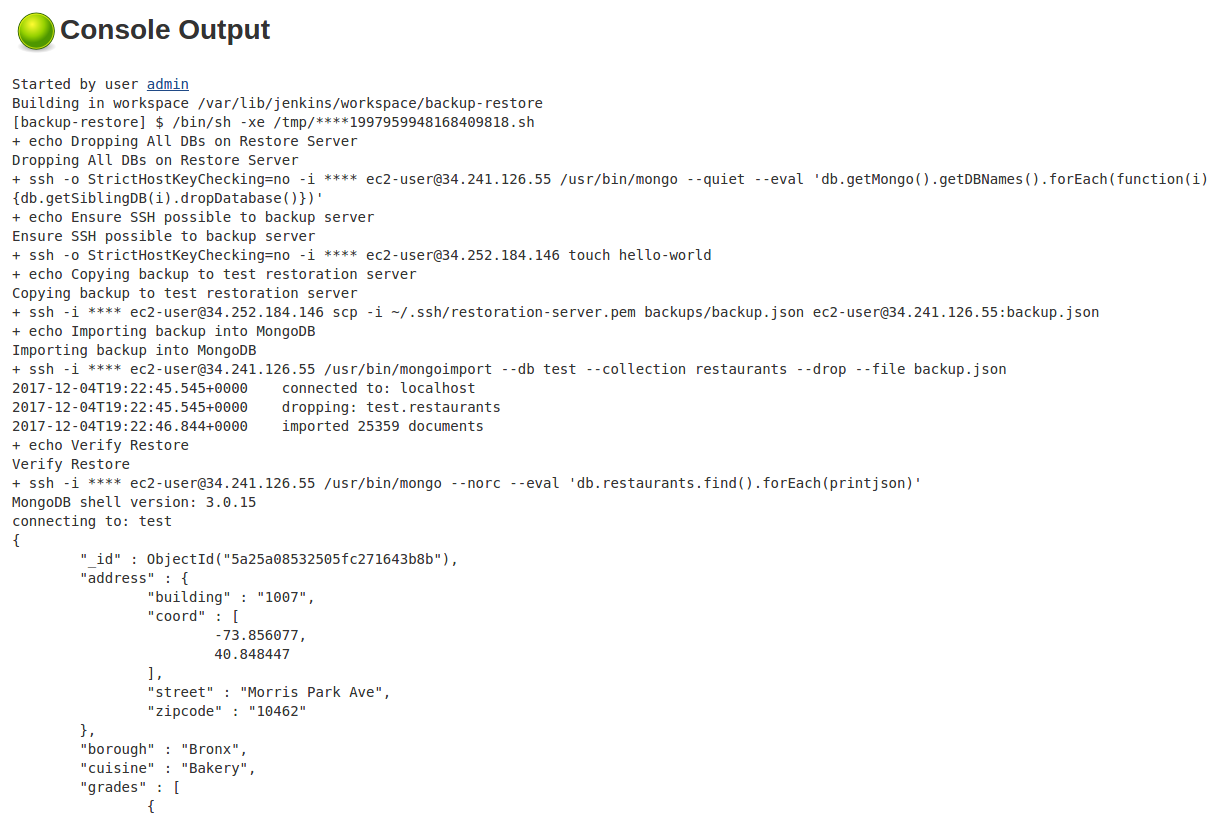
\includegraphics[width=\textwidth,keepaspectratio]{poc1}
		\label{fig:poc1}
	\end{figure}
	
	\subsubsection{Issues Encountered}
	In order to move the backup securely from the \textit{backup} server to the \textit{restoration} server the correct SSH credentials were needed. These were securely implemented in Jenkins using the \hyperref[creds-plugin]{aforementioned} Credentials Plugin. This allows Jenkins to securely communicate with both servers.
	
	\begin{figure}[H]
		\caption{SSH Credentials Stored in Jenkins}
		\centering
		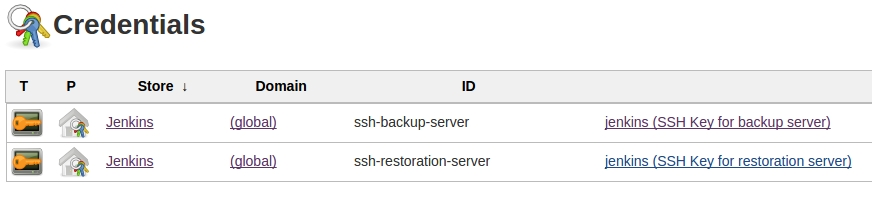
\includegraphics[width=\textwidth,keepaspectratio]{creds}
		\label{fig:creds}
	\end{figure}

	\subsubsection{Results}
	The POC showed backups can be successfully transported to and imported into a remote server. Once imported, a successful \textit{findAll} command proves that the data is still readable. Although, reading all entries and printing to the console may not be a practical solution it satisfies the POC in that it proves the backup can be restored and validated. During development, this POC can be improved in the following areas:
	\begin{itemize}
		\item Rudimentary validation: Reading all entries my be impractical for large backups;
		\item Security: Printing the DB entries to the Jenkins console may not be desirable;
		\item Automation: This implementation used the pre-existing \textit{restoration} server. Setup and tear-down of this should be automated using \hyperref[aws-cli]{AWS CLI}.
	\end{itemize}
		
	\subsection{\ref{poc2} User Rules}
	This POC was tested by creating a basic frontend with React which uses Jenkins API to trigger an arbitrary Jenkins Job. The frontend code to trigger a Jenkins job is shown in \autoref{fig:jenkins-api}
	
	\begin{figure}[H]
		\caption{Use of Jenkins API in React Web App}
		\centering
		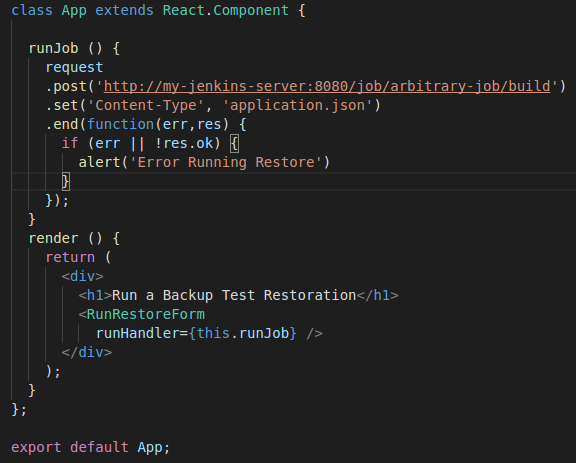
\includegraphics[width=\textwidth,keepaspectratio]{jenkins-api}
		\label{fig:jenkins-api}
	\end{figure}
	
	\subsubsection{Issues Encountered}
	For the purposes of the POC, the web app was run in a local \textit{npm} development environment whereas the Jenkins server was running in AWS. Accordingly, API calls from the app to the external domain where Jenkins was running were blocked. This was due to Cross Origin Resource Sharing (CORS). 
	
	CORS comes from the \textit{same-origin policy} observed by web browser.  It prevents JavaScript from making API request to different origins to the one in which it is running. This is for security reasons \citep{mozilla}. Thus, the API calls failed because CORS was not enabled. 
	
	In order to overcome this issue, a Jenkins plugin for enabling CORS was installed. As shown \autoref{fig:cors}, this plugin allows whitelisting of requests based on IP (Access-Control-Allow-Origins) and HTTP method (Access-Control-Allow-Headers), for example. 
	\begin{figure}[H]
		\caption{CORS Plugin}
		\centering
		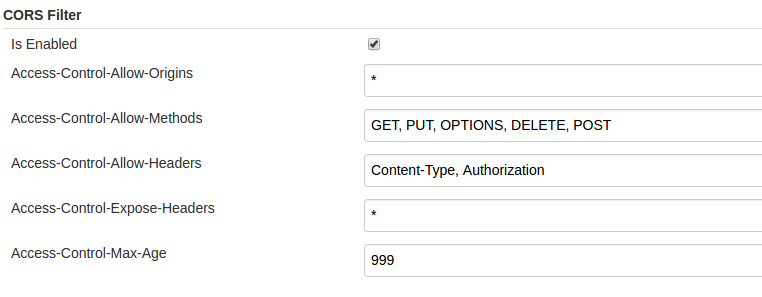
\includegraphics[width=\textwidth,keepaspectratio]{cors}
		\label{fig:cors}
	\end{figure}
		
	
	\subsubsection{Results}
	This POC showed that implementation of Jenkins jobs can be abstracted from the user therefore allowing the system to present the user with a simple form to complete in order to commence an automated restoration. During development this, POC can be further developed in the following areas:
	\begin{itemize}
		\item Job Creation: Create jobs (such as scheduled restore) using the Jenkins API;
		\item Frontend: Further develop the frontend. 
	\end{itemize}
	
	\subsection{\ref{poc3} Security}
	This POC utilised the same setup as \hyperref[poc1]{POC1}. In this instance the Jenkins job copied an encrypted backup to the \textit{restoration} server. The backup is then decrypted using GPG and a private key on the \textit{restoration} server and the contents printed to verify decryption. This is shown in \autoref{fig:decrypt}.
	
	\begin{figure}[H]
		\caption{Backup File Decryption}
		\centering
		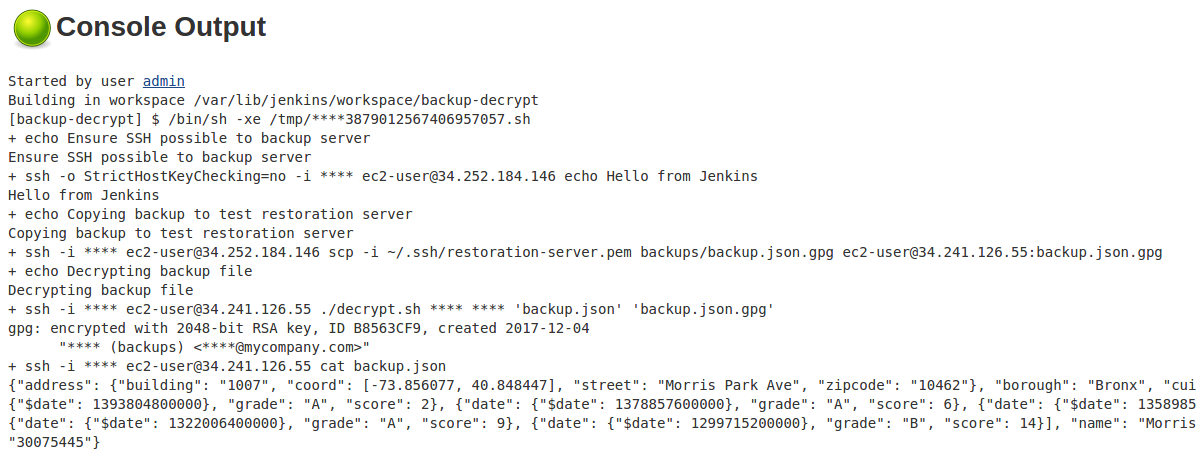
\includegraphics[width=\textwidth,keepaspectratio]{decrypt}
		\label{fig:decrypt}
	\end{figure}
	
	\subsubsection{Issues Encountered}
	As GPG keys are managed by keyrings they cannot be stored in Jenkins using the Credentials plugin nor can they be used to decrypt remote files. For this reason, the GPG key was imported into a keyring on the \textit{restoration} server. This enabled successful decryption of the file.
	
	\subsubsection{Results}
	Although the use of the keys was not implemented as originally planned, this POC demonstrated that the system in it's current architecture can successfully copy an encrypted backup file to the \textit{restoration} server where it is decrypted. During development some aspects of this implementation can be explorer further:
	\begin{itemize}
		\item Security: Automating the provision and destruction of the \textit{restoration} server will ensure that the private key is not left unnecessarily on servers in the cloud. 
	\end{itemize}
	